
\section{不动点与 \texorpdfstring{$\mathcal{D}$}{D} 上的\trGeodesic}
\label{sec:fixed-points-geodesics}

\hzsync{theorem}{11}%
\hzsync{proposition}{17}%
\hzsync{lemma}{12}%
\hzsync{equation}{34}%

正如我们所证明的，$\mathcal{D}$ 中的一个\trSymplecticDiffeomorphism{} $\varphi$%
拥有一个由\trMinimax{}原理所保证的特定\trFixedPoint{} $x=\varphi(x)$。其%
\trAction{}满足 $A(x,\varphi)=\gamma(\varphi)$。\textbf{\trPeriodic{}点}%
（periodic point）是 $\varphi$ 更高次迭代的诸不动点 $x=\varphi^{N}(x)$，而我们%
把有限集
\[
\mathcal{O}(x)=\bigl\{x,\ \varphi(x),\ \varphi\bigl(\varphi(x)\bigr),\ \ldots,\ %
\varphi^{N}(x)=x\bigr\}
\]
称为 $x$ 的\trOrbit。下述定性存在性\trhTheorem{}出自 C.~\trViterbo{} [218]。

\begin{theorem}\label{thm:viterbo-periodic-points}
每个 $\varphi\in\mathcal{D}^{-}\setminus\{\id\}$ 都拥有无穷多个\trPeriodic{}点%
$x_{j}=\varphi^{j}\bigl(x_{j}\bigr)$，它们具有正的\trAction
\[
A\bigl(x_{j},\varphi^{j}\bigr)\ \geq\ \gamma(\varphi)\ >\ 0
\]
以及两两不交的\trOrbit
\[
\mathcal{O}\bigl(x_{j}\bigr)\cap\mathcal{O}\bigl(x_{k}\bigr)=\varnothing,\qquad%
k\neq j\ .
\]
该陈述对 $\varphi\in\mathcal{D}^{+}\setminus\{\id\}$ 也成立。事实上，利用他在%
$\R^{2n}$ 中一个特殊\trCapacity{}的同调版本，C.~\trViterbo{}证明了一个更一般的%
陈述，其中只假定 $\varphi\in\mathcal{D}$ 满足 $\varphi\neq\id$。
\end{theorem}

\begin{proof}
依据对 $\varphi$ 的假设，我们可以找到 $H\in\mathcal{H}$，满足 $\varphi=\varphi_{H}$、%
$H\leq0$ 且 $H\neq0$。于是依据\cref{prop:gamma-on-d}有 $\gamma(\varphi)>0$。由于对%
某个\trBounded{}开集 $U$ 有 $\operatorname{supp}(H)\subset[0,1]\times U$，我们便有
\[
0<\gamma(\varphi)\leq e(U)\ .
\]
的确，若 $\psi\in\mathcal{D}$ 满足 $\psi(U)\cap U=\varnothing$，则依据%
\cref{prop:gamma-le-energy}%
有 $\gamma(\varphi)\leq E(\psi)$，从而 $\gamma(\varphi)\leq e(U)$。由于%
$\varphi\leq\id$，利用 $\gamma$ 的\trMonotonicity，我们得到估计
\[
0<\gamma(\varphi)\leq\gamma\bigl(\varphi^{2}\bigr)\leq\ldots\leq%
\gamma\bigl(\varphi^{j}\bigr)\leq e(U)
\]
它对 $\varphi$ 的一切迭代成立。对每个 $j$ 都存在满足 $\gamma\bigl(\varphi^{j}\bigr)=A\bigl(x_{j},\varphi^{j}\bigr)%
\geq\gamma(\varphi)>0$ 的\trFixedPoint{} $x_{j}=\varphi^{j}\bigl(x_{j}\bigr)$，剩下%
的只须证明它们之中有无穷多个属于两两不交的\trPeriodicOrbit。为看清这一点，注意：%
若对某个 $l$ 有 $x_{k}=\varphi^{l}\bigl(x_{j}\bigr)$（$j\neq k$），则如计算所表明的，\footnote{原书印作「$=lA\bigl(x_{j},\varphi^{j}\bigr)=l\gamma\bigl(\varphi^{j}\bigr)$」，倍率 $l$ 只是沿轨道的平移迭代数，与作用量按迭代次数的缩放无关：设该轨道的最小周期 $m$ 整除 $j$ 与 $k$，取迭代 Hamiltonian $H_{j}(t,x)=j\,H(jt,x)$ 计算便得 $A\bigl(x,\varphi^{j}\bigr)=\tfrac{j}{m}\int_{0}^{m}\Bigl[\tfrac{1}{2}\bigl\langle-J\dot{x},x\bigr\rangle-H\bigl(s,x(s)\bigr)\Bigr]ds$，故正确倍率为 $\tfrac{k}{j}$，此处径改。——译者注}
\[
\gamma\bigl(\varphi^{k}\bigr)=A\bigl(x_{k},\varphi^{k}\bigr)=\frac{k}{j}A\bigl(x_{j},\varphi^{j}\bigr)=%
\frac{k}{j}\gamma\bigl(\varphi^{j}\bigr)\ \geq\ \frac{k}{j}\gamma(\varphi),
\]
于是，倘若诸 $x_{j}$ 只属于有限多条\trPeriodicOrbit，便有一条轨道容纳无穷多个 $x_{j}$；固定其中一个指标 $j$ 而令 $k$ 沿该轨道任意增大，上式即与界 $\gamma\bigl(\varphi^{k}\bigr)\leq e(U)$ 相矛盾。故该\trhTheorem{}随之得证。
\end{proof}

若不依赖时间的\trHamiltonianFunction{} $H\in C^{\infty}_{c}\bigl(\R^{2n}\bigr)$ 不%
恒为零，则正如我们在第 4 章中所看到的，\trHamiltonianSystem{} $\dot{x}=X_{H}(x)$%
在 $H$ 的诸正则\trEnergySurface{}上拥有许多\trPeriodicSolution。然而，关于这些解的%
周期人们一无所知，因而我们想对快速\trPeriodicSolution{}补充一个定性的存在性陈述。%
回顾：若 $H\in C^{\infty}_{c}(U)$ 满足 $\lVert H\rVert>c_{0}(U)$，则只要 $H\leq0$%
且在一个开子集上 $H=\inf H$，系统 $\dot{x}=X_{H}(x)$ 便拥有一个周期含于区间%
$0<T\leq1$ 之内的非常值 $T$-\trPeriodicSolution。这可从\trCapacity{} $c_{0}(U)$ 的%
定义直接推得。将此陈述推广，我们将证明：

\begin{theorem}\label{thm:fast-periodic-solutions}
设 $H\in C^{\infty}_{c}(U)$ 不恒为零。则\trHamiltonianSystem{} $\dot{x}=X_{H}(x)$%
具有满足 $0<T\leq T^{*}$ 的非常值 $T$-\trPeriodicSolution，其中
\[
T^{*}\ >\ \frac{c_{0}(U)}{\lvert H\rvert_{C^{0}}}\ .
\]
\end{theorem}

\begin{proof}
利用第 3 章\footnote{原书印作「Chapter 5」，容量 $c_{0}$ 之论证出自第 3 章，疑为「Chapter 3」之误，此处径改。——译者注}中的论证，本证明将可直接由\trCapacity{} $c_{0}$ 的定义得到。令%
$H^{+}=\max H$、$H^{-}=-\min H$，则 $\lvert H\rvert_{C^{0}}$\footnote{原书下标印作 $C^{o}$（字母 $o$），疑为 $C^{0}$（数字零）之误，此处径改。——译者注}$=\max\bigl\{H^{+},H^{-}\bigr\}$。%
设 $H^{+}\geq H^{-}$，则因 $H\not\equiv0$ 有 $H^{+}>0$。取 $\varepsilon>0$ 充分小，%
使得 $T^{*}\bigl(H^{+}-\varepsilon\bigr)>c_{0}(U)$。再选取一个\trSmooth{}函数%
$f:\R\to[0,\infty)$，满足：当 $s\leq0$ 时 $f(s)=0$，当 $s\geq H^{+}$ 时%
$f(s)=H^{+}-\varepsilon$，并且 $0\leq f'(s)\leq1$。然后如下定义%
\trHamiltonianFunction{} $K$：
\[
K\ =\ T^{*}f\circ H\ .
\]
由于 $\lVert K\rVert>c_{0}(U)$，方程
\[
\dot{x}=X_{K}(x)=T^{*}f'(H)X_{H}(x)
\]
便拥有周期为 $0<\tau\leq1$ 的非常值 $\tau$-\trPeriodicSolution{} $x(t)$。函数%
$T^{*}f'\bigl(H\bigl(x(t)\bigr)\bigr)=c$ 是一个正常数，故 $y(t)=x\bigl(\tfrac{1}{c}t\bigr)$%
是 $\dot{y}=X_{H}(y)$ 的一个\trPeriodicSolution，其周期为 $c\tau\leq T^{*}$。同样的%
论证适用于 $H^{-}\geq H^{+}$ 的情形，陈述得证。
\end{proof}

对一条\trSmooth{}弧 $\varphi^{t}:[a,b]\to\mathcal{D}$，我们如下赋予其长度：
\[
\operatorname{length}\bigl(\varphi^{[a,b]}\bigr)\ =\ \int_{a}^{b}\Bigl[\sup_{x}H_{t}-%
\inf_{x}H_{t}\Bigr]dt\ .
\]
函数 $H$ 是 $[a,b]\times\R^{2n}$ 上生成该弧的唯一\trCompactSupport\trSmooth{}函数，%
它由 $\bigl(\frac{d}{dt}\varphi^{t}\bigr)\circ\bigl(\varphi^{t}\bigr)^{-1}(x)=J\nabla H(t,x)$%
（$a\leq t\leq b$）确定。于是在\trMetric{}空间 $(\mathcal{D},d)$ 中，我们把一条%
\trSmooth\trPath{} $\varphi^{t}:[a,b]\to\mathcal{D}$ 称为\trGeodesic，如果局部地%
看，它的长度就是端点之间的最短连接；也就是说，如果
\[
\operatorname{length}\bigl(\varphi^{[t,s]}\bigr)=d\bigl(\varphi^{t},\varphi^{s}\bigr)
\]
对一切使 $\lvert t-s\rvert$ 充分小的 $a\leq t<s\leq b$ 成立。\trGeodesic{}的例子便是%
不依赖时间的\trHamiltonianFunction{} $H\in C^{\infty}_{c}\bigl(\R^{2n}\bigr)$ 的诸%
\trFlow，下面我们将证明这一点。在此情形，由定义可得
\[
\operatorname{length}\bigl(\varphi_{H}^{[s,t]}\bigr)=\lvert t-s\rvert\cdot\lVert H\rVert\ .
\]

\begin{proposition}\label{prop:autonomous-geodesic}
若 $H\in C^{\infty}_{c}\bigl(\R^{2n}\bigr)$ 不依赖时间，则\trFlow{}%
$\varphi^{t}=\varphi_{H}^{t}$ 是 $\mathcal{D}$ 中的一条\trGeodesic，并且对一切满足%
$\lvert t-s\rvert<2\pi/h$ 的 $t<s$ 还满足
\[
d\bigl(\varphi^{t},\varphi^{s}\bigr)=\lvert t-s\rvert\cdot\lVert H\rVert=%
\operatorname{length}\bigl(\varphi^{[t,s]}\bigr)
\]
其中 $h:=\sup_{x}\lvert H_{xx}\rvert$。
\end{proposition}

\begin{proof}
我们先回顾：对不依赖时间的\trVectorField，若周期太小，其 $T$-\trPeriodicSolution{}%
必定是常值解。的确，设 $x(t)$ 是 $\dot{x}=X_{H}(x)$ 的一个 $T$-\trPeriodicSolution。%
把周期规范化，我们定义 $y(t)=x(tT)$，它求解
\[
\dot{y}=X_{TH}(y),\qquad\text{且}\ y(0)=y(1)\ .
\]
注意：对 $\R^{2n}$ 中每个平均值为零的 1-周期\trLoop{} $z$，我们有 $L^{2}$-\trEstimate%
$\lVert z\rVert\leq\frac{1}{2\pi}\lVert\dot{z}\rVert$。这从\trFourier{}级数即可看出。%
把这个观察应用于其平均值为零的 $\dot{y}$，我们可以估计
\[
\lVert\dot{y}\rVert\ \leq\ \frac{1}{2\pi}\lVert\ddot{y}\rVert\ =\ \frac{1}{2\pi}T\cdot%
\bigl\lVert H_{xx}\bigl(y(t)\bigr)\dot{y}\bigr\rVert\ \leq\ \frac{Th}{2\pi}\lVert\dot{y}\rVert,
\]
由此，当 $hT<2\pi$ 时便得 $\dot{y}=0$，于是 $y(t)=y(0)$ 是常值解。从而，当%
$hT<2\pi$ 时，我们从\cref{prop:time-independent-energy}%
得出 $E\bigl(\varphi_{TH}\bigr)=T\lVert H\rVert$。于是，设%
$\lvert t-s\rvert<2\pi/h$，我们便可以如下计算这个\trDistance：
\begin{align*}
d\bigl(\varphi^{s},\varphi^{t}\bigr)\ &=\ E\bigl(\bigl(\varphi^{s}\bigr)^{-1}\circ\varphi^{t}\bigr)\\
&=\ E\bigl(\varphi_{H}^{\,t-s}\bigr)=E\bigl(\varphi_{(t-s)H}\bigr)=\lvert t-s\rvert\,\lVert H\rVert,
\end{align*}
正如该\trhProposition{}所断言的。
\end{proof}

显然，对自治\trHamiltonianFunction，只要 $\varphi^{t}$ 不容有非平凡\trFixedPoint，%
就有
\[
d\bigl(\varphi^{t},\id\bigr)=t\lVert H\rVert=\operatorname{length}\bigl(\varphi^{[0,t]}\bigr)
\]
按定义，$\mathcal{D}$ 中的一条\trGeodesic{}局部地使曲线的长度最小。整体上这未必%
成立，正如下面的例子所表明的。

\begin{proposition}\label{prop:geodesic-length-gap}
对每个 $\varepsilon>0$，都存在 $\mathcal{D}$ 中一条\trGeodesic{} $\varphi^{t}$%
（$0\leq t\leq1$），它从 $\varphi^{0}=\id$ 出发，并且对一切 $0\leq t\leq1$ 满足
\[
d\bigl(\varphi^{t},\id\bigr)\leq\varepsilon\quad\text{且}\quad%
\operatorname{length}\bigl(\varphi^{[0,t]}\bigr)\geq\frac{t}{\varepsilon}\ .
\]
\end{proposition}

\begin{proof}
取原点的一个满足 $16\,e(U)<\varepsilon$ 的开\trNeighborhood{} $U$，并选取一个不依赖%
时间的 $H\in C^{\infty}_{c}(U)$ 使 $\lVert H\rVert>1/\varepsilon$。于是，依据%
\trSikorav{}的估计，当 $0\leq t\leq1$ 时我们得到 $d\bigl(\varphi^{t},\id\bigr)=%
E\bigl(\varphi_{tH}\bigr)\leq16\,e(U)<\varepsilon$，而 $\operatorname{length}%
\bigl(\varphi^{[0,t]}\bigr)=t\lVert H\rVert\geq t/\varepsilon$，正如所断言。
\end{proof}

我们特别地看到，\trMetric{}空间 $(\mathcal{D},d)$ 不是一个\textbf{「\trFlat{}」}%
（flat）空间。然而「局部地」，空间 $(\mathcal{D},d)$ 却是「\trFlat{}」的。这最近由%
M.~\trBialy{}与 L.~\trPolterovich{} [22] 证明，他们给出了 $(\mathcal{D},d)$ 中%
\trGeodesic{}的一个完整描述，我们接下来将介绍它。为避免病态情形，我们只考察%
正则的\trSmooth\trPath{} $g:I\to\mathcal{D}$，其中 $I\subset\R$ 为一个区间。这要求%
生成\trPath{} $g$ 的\trHamiltonianFunction{} $H:I\times\R^{2n}\to\R$ 满足%
$\lVert H_{t}\rVert\neq0$（$t\in I$）。回顾：$H_{t}(x)=H(t,x)$，并且如上所述
\[
\lVert H_{t}\rVert\ =\ \max_{x}H_{t}(x)\ -\ \min_{x}H_{t}(x)\ .
\]

\begin{definition}\label{def:minimal-geodesic}
一条正则\trSmooth\trPath{} $g:I\to\mathcal{D}$ 称为\textbf{\trMinimal\trGeodesic}%
（minimal geodesic），如果对 $I$ 中满足 $a<b$ 的一切 $a$ 与 $b$，都有
\[
\operatorname{length}\bigl(g|_{[a,b]}\bigr)\ =\ d\bigl(g(a),g(b)\bigr)\ .
\]
\end{definition}

回顾：长度定义为
\[
\operatorname{length}\bigl(g|_{[a,b]}\bigr):=\int_{a}^{b}\lVert H_{t}\rVert\,dt\ ,
\]
其中 $H\in\mathcal{H}$ 生成\trPath{} $g$。从而，$g:I\to\mathcal{D}$ 是一条\trGeodesic%
，如果对每个 $c\in I$ 都存在区间 $I_{c}\subset I$，使得 $g:I_{c}\to\mathcal{D}$%
是一条\trMinimal\trGeodesic。为了借生成\trHamiltonianFunction{}来刻画\trGeodesic，下述由%
[22] 引入的概念被证明是有用的。

\begin{definition}\label{def:quasi-autonomous}
一个\trSmooth\trHamiltonianFunction{} $H:I\times\R^{2n}\to\R$ 称为\textbf{\trQuasiAutonomous}%
（quasi-autonomous）的，如果存在两点 $x_{+}$、$x_{-}\in\R^{2n}$ 使得
\begin{align*}
\max_{x}H_{t}(x)\ &=\ H\bigl(t,x_{+}\bigr)\qquad&&\text{对一切}\ t\in I\\
\min_{x}H_{t}(x)\ &=\ H\bigl(t,x_{-}\bigr)\qquad&&\text{对一切}\ t\in I\ .
\end{align*}
相应地，$I\times\R^{2n}$ 上的一个函数 $H$ 称为\textbf{局部\trQuasiAutonomous}%
（locally quasi-autonomous）的，如果对每个 $c\in I$ 都存在区间 $I_{c}\subset I$，%
使得 $H$ 在 $I_{c}\times\R^{2n}$ 上是\trQuasiAutonomous{}的。特殊的例子当然是自治%
\trHamiltonianFunction。
\end{definition}

以 $\mathcal{C}=C^{\infty}_{c}\bigl(\R^{2n}\bigr)$\footnote{原书印作「$R^n$」，疑为 $R^{2n}$ 之误，此处径改。——译者注} 表示自治\trHamiltonianFunction{}%
的\trLinear{}空间，其上装备与范数 $\lVert H\rVert=\max H-\min H$ 相伴的\trMetric。我们把%
一条正则\trSmooth{}弧 $f:I\to\mathcal{C}$ 称为 $\mathcal{C}$ 的\trMinimal\trGeodesic，如果对%
$I$ 中每个 $a<b$ 都有
\[
\lVert f(b)-f(a)\rVert\ =\ \int_{a}^{b}\Bigl\lVert\frac{d}{ds}f(s)\Bigr\rVert\,ds\ .
\]
在此术语下，依据下文的\cref{lem:quasi-autonomous-integral}，一个\trHamiltonianFunction{}%
$H\in\mathcal{H}$ 是\trQuasiAutonomous{}的，当且仅当它是 $\mathcal{C}$ 中一条\trGeodesic{}弧的时间导数。

下述\trhTheorem{}推广了\cref{prop:autonomous-geodesic}，并给出 $(\mathcal{D},d)$ 上诸%
\trGeodesic{}的一个完整描述。

\begin{theorem}[\trBialy-\trPolterovich]\label{thm:geodesic-characterization}
一条正则\trSmooth\trPath{} $g:I\to\mathcal{D}$ 是\trGeodesic，当且仅当它由一个局部\trQuasiAutonomous%
\trHamiltonianFunction{}所生成。
\end{theorem}

本节其余部分将用于该\trhTheorem{}的证明。这个结果将从\trMinimal\trGeodesic{}的一个判据%
推出，我们先表述这个判据。回顾：在 5.2 节中我们已为\trMapping{} $\varphi\in\mathcal{D}$%
配上了\trActionSpectrum{} $\sigma(\varphi)=\bigl\{A(x,\varphi)\ \bigm|\ %
x\in\operatorname{Fix}(\varphi)\bigr\}$。正如我们在\cref{prop:spectrum-compact}中所%
看到的，\trActionSpectrum{}是一个\trCompact{}且\trNowhereDense{}的集合。一般地说，它并%
不连续地依赖于 $\varphi$。对一条\trSmooth\trPath{} $g:[a,b]\to\mathcal{D}$，有属于它的一个%
\textbf{\trBifurcation{}图}（bifurcation diagram）$\Sigma(g)$。它定义为集合
\[
\Sigma(g):=\bigl\{(t,s)\in\R^{2}\ \bigm|\ a<t\leq b\ \text{且}\ %
s\in\sigma\bigl(g(t)g(a)^{-1}\bigr)\bigr\}\ .
\]
若\trPath{} $g:[a,b]\to\mathcal{D}$ 由\trQuasiAutonomous\trHamiltonianFunction{} $H$ 生成，则对每个%
$a\leq t\leq b$，我们都有属于 $\operatorname{Fix}\bigl(g(t)g(a)^{-1}\bigr)$ 的两个特定%
\trFixedPoint{} $x_{+}$、$x_{-}$。它们的\trAction{}是由
\[
\gamma_{+}(t)\ =\ -\int_{a}^{t}H_{t}\bigl(x_{-}\bigr)\,dt\ ,\qquad
\gamma_{-}(t)\ =\ -\int_{a}^{t}H_{t}\bigl(x_{+}\bigr)\,dt\ .
\]
所定义的函数 $\gamma_{+}$、$\gamma_{-}:[a,b]\to\R$。注意 $\gamma_{-}(t)\leq0\leq\gamma_{+}(t)$。%
相应的图像 $\Gamma_{\pm}(t)=(t,\gamma_{\pm}(t))$ 是\trBifurcationDiagram{}中两条连续的特定\trCurve。当然，%
由于所考察的诸\trHamiltonianFunction{}都具有\trCompactSupport，\trCurve{}%
$\Gamma(t)=(t,0)$ 总是含于 $\Sigma(g)$ 之中。

\begin{definition}\label{def:simple-diagram}
考察由\trQuasiAutonomous\trHamiltonianFunction{}生成的一条正则\trPath{} $g:[a,b]\to\mathcal{D}$。称它的%
\trBifurcationDiagram{} $\Sigma(g)$ 为\textbf{\trSimple}（simple）的，如果下列条件成立：
(i) 每当 $\gamma_{+}(t)$ 不恒为零，对每个 $\tau>a$ 下述结论成立：不存在连续\trCurve{}%
$(t,u(t))\subset\Sigma(g)$（$\tau\leq t\leq b$）把点 $(\tau,u(\tau))\in\Gamma_{+}(\tau)$%
与一个满足 $\gamma_{-}(b)<u(b)<\gamma_{+}(b)$ 的点 $(b,u(b))$ 连接起来。
(ii) 类似地，对每个 $\tau>a$，每当 $\gamma_{-}(t)$ 不恒为零，我们要求：不存在连续%
\trCurve{} $(t,u(t))\subset\Sigma(g)$（$\tau\leq t\leq b$）把 $(\tau,u(\tau))\in%
\Gamma_{-}(\tau)$ 与满足 $\gamma_{-}(b)<u(b)<\gamma_{+}(b)$ 的 $(b,u(b))$ 连接起来。
\end{definition}

图 5.10 中的第一幅小图描绘了一个不\trSimple{}的图。第二幅小图则属于一条正则\trPath%
$g:[0,b]\to\mathcal{D}$：为简单计，它从\trIdentityMap{}出发，其生成%
\trHamiltonianFunction{} $H$ 不依赖时间 $t$，并且它不容有任何非常值的\trPeriodicOrbit。%
在这个例子中，诸\trFixedPoint{}是 $H$ 的\trCriticalPoint{} $x$，其\trAction{}是直线
\[
A\bigl(x,g(t)\bigr)\ =\ -\int_{0}^{t}H(x)\,dt\ =\ -tH(x)\ .
\]
相应的\trBifurcation{}图是\trSimple{}的，因为 $H$ 的诸\trCritical{}水平是\trNowhereDense{}的。

\begin{theorem}[\trBialy-\trPolterovich]\label{thm:simple-diagram-geodesic}
设正则\trSmooth\trPath{} $g:I\to\mathcal{D}$ 由一个\trQuasiAutonomous\trHamiltonianFunction{}生成。若%
\trBifurcation{}图 $\Sigma(g)$ 是\trSimple{}的，则 $g$ 是一条\trMinimal\trGeodesic。
\end{theorem}

\noindent\begin{minipage}{\linewidth}
\centering
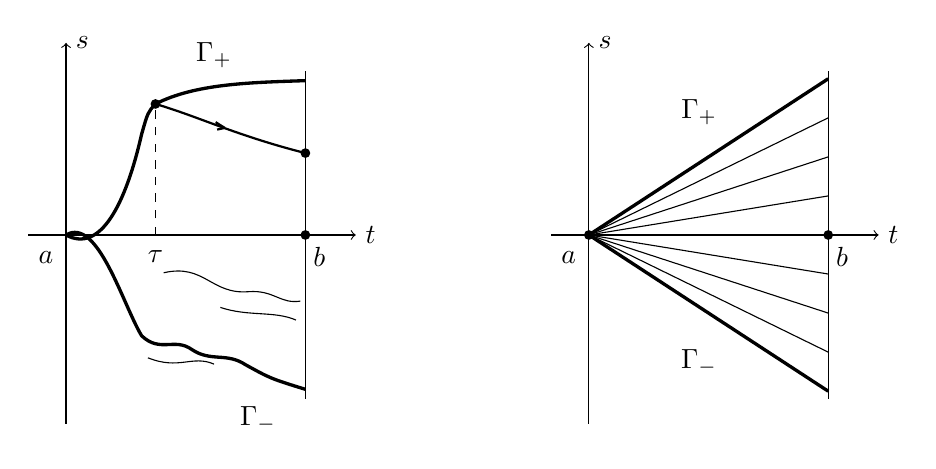
\begin{tikzpicture}[scale=0.8]
  \begin{scope}
    \draw[->] (0,-3.0) -- (0,3.05) node[right] {$s$};
    \draw[->] (-0.6,0) -- (4.6,0) node[right] {$t$};
    \draw (3.8,-2.6) -- (3.8,2.6);
    \draw[very thick] (0,0) .. controls (0.55,-0.30) and (0.95,0.50)
        .. (1.20,1.60) .. controls (1.30,1.95) .. (1.42,2.08);
    \draw[very thick] (1.42,2.08) .. controls (2.05,2.40) and (2.90,2.42) .. (3.8,2.45);
    \fill (1.42,2.08) circle (2.2pt);
    \draw[thick] (1.42,2.08) .. controls (2.10,1.88) and (2.70,1.58) .. (3.8,1.30);
    \draw[thick] (2.52,1.70) -- (2.375,1.791);
    \draw[thick] (2.52,1.70) -- (2.399,1.673);
    \fill (3.8,1.30) circle (2.2pt);
    \draw[dashed] (1.42,0) -- (1.42,2.08);
    \node at (1.42,-0.34) {$\tau$};
    \draw[very thick] (0,0) .. controls (0.50,0.30) and (0.90,-1.10)
        .. (1.20,-1.60) .. controls (1.50,-1.88) and (1.72,-1.62)
        .. (2.00,-1.82) .. controls (2.30,-2.02) and (2.55,-1.86)
        .. (2.85,-2.06) .. controls (3.25,-2.28) .. (3.8,-2.45);
    \draw[thin] (1.55,-0.60) .. controls (2.20,-0.45) and (2.30,-0.95)
        .. (2.90,-0.90) .. controls (3.30,-0.87) and (3.40,-1.10) .. (3.72,-1.05);
    \draw[thin] (1.30,-1.95) .. controls (1.80,-2.15) and (2.00,-1.90) .. (2.35,-2.05);
    \draw[thin] (2.45,-1.15) .. controls (2.90,-1.30) and (3.30,-1.20) .. (3.65,-1.35);
    \node at (2.35,2.85) {$\Gamma_{+}$};
    \node at (3.05,-2.92) {$\Gamma_{-}$};
    \node at (-0.32,-0.36) {$a$};
    \node at (4.02,-0.34) {$b$};
    \fill (3.8,0) circle (2.2pt);
  \end{scope}
  \begin{scope}[shift={(8.3,0)}]
    \draw[->] (0,-3.0) -- (0,3.05) node[right] {$s$};
    \draw[->] (-0.6,0) -- (4.6,0) node[right] {$t$};
    \draw (3.8,-2.6) -- (3.8,2.6);
    \foreach \y in {0.62,1.24,1.86} {%
      \draw[thin] (0,0) -- (3.8,\y);
      \draw[thin] (0,0) -- (3.8,-\y);}
    \draw[very thick] (0,0) -- (3.8,2.48);
    \draw[very thick] (0,0) -- (3.8,-2.48);
    \node at (1.75,1.95) {$\Gamma_{+}$};
    \node at (1.75,-2.02) {$\Gamma_{-}$};
    \fill (0,0) circle (2.2pt);
    \fill (3.8,0) circle (2.2pt);
    \node at (-0.32,-0.36) {$a$};
    \node at (4.02,-0.34) {$b$};
  \end{scope}
\end{tikzpicture}

图 5.10
\end{minipage}

\begin{proof}
该证明基于上文 5.3 节中引入的特定映射 $\gamma:\mathcal{D}\to\R$ 的诸性质。这个映射%
特别地是连续的，从而定义了\trBifurcation{}图的一个连续\trSection。为简化论述，我们设%
$I=[0,1]$ 且 $g(0)=\id$。关键的一步是下述推广了\cref{prop:time-independent-energy}%
的\trhLemma。

\begin{lemma}\label{lem:gamma-endpoints}
设 $H$ 是\trQuasiAutonomous{}的，并且生成一条具有\trSimple{}的\trBifurcation{}图 $\Sigma(g)$ 的\trPath%
$g:[0,1]\to\mathcal{D}$。则
\[
\gamma\bigl(g(1)\bigr)=\gamma_{+}(1),\qquad\gamma\bigl(g(1)^{-1}\bigr)=-\gamma_{-}(1)\ .
\]
\end{lemma}

\begin{proof}
回顾：依据\cref{lem:gamma-real}，对一切 $t$ 有 $\gamma_{-}(t)\leq\gamma\bigl(g(t)\bigr)%
\leq\gamma_{+}(t)$。我们先证明：当 $\tau>0$ 充分小时 $\gamma\bigl(g(\tau)\bigr)=%
\gamma_{+}(\tau)$。通过\trReparametrization，我们对 $0\leq t\leq1$ 与 $\tau>0$ 引入%
$F(t,x)=\tau H(\tau t,x)$。我们可以设 $x_{-}=0$，于是当 $\tau$ 充分小时%
$F(t,x)\leq F(t,0)+\pi\lvert x\rvert^{2}$。仿照\cref{prop:gamma-sign}之证明进行，我们%
利用 $\gamma$ 的\trMonotonicity{}并估计
\[
\gamma\bigl(g(\tau)\bigr)\ =\ \gamma(F)\ \geq\ -\int_{0}^{1}F(t,0)\,dt\ =\ %
-\int_{0}^{\tau}H(t,0)\,dt\ =\ \gamma_{+}(\tau)\ .
\]
于是如所断言，$\gamma\bigl(g(\tau)\bigr)=\gamma_{+}(\tau)$。类似地，只要 $\tau$ 充分小，%
便有 $\gamma\bigl(g(\tau)^{-1}\bigr)\geq-\gamma_{-}(\tau)$。对 $t=1$ 的诸论断现在由对%
$\Sigma(g)$ 的假设推出。的确，若 $\gamma_{+}(t)\equiv0$，则 $H(t,x)\geq0$，从而由%
$\gamma$ 的\trMonotonicity{}（\cref{prop:gamma-sign}）得 $\gamma\bigl(g(1)\bigr)=0$，%
正如所愿。现设 $\gamma_{+}(t)\not\equiv0$。用反证法，我们设%
$\gamma\bigl(g(1)\bigr)<\gamma_{+}(1)$，并断言%
$\gamma_{-}(1)<\gamma\bigl(g(1)\bigr)<\gamma_{+}(1)$。的确，若 $\gamma_{-}(1)\equiv0$，%
则 $H(t,x)\leq0$，从而由\cref{prop:gamma-sign}得 $\gamma\bigl(g(1)\bigr)>0$。若%
$\gamma_{-}(1)<0$，我们只须注意 $\gamma\geq0$，断言便得证。现在考察由连续函数%
$u(t)=\min\bigl\{\gamma\bigl(g(t)\bigr),\gamma_{+}(t)\bigr\}$（$\tau\leq t\leq1$）%
定义的图像 $\Gamma$。则 $\Gamma\subset\Sigma(g)$，而这与 $\Sigma(g)$ 所要求的\trSimplicity{}相%
矛盾。我们已证明该\trhLemma{}中的第一个论断；类似地可得第二个论断。
\end{proof}

现在，依据\cref{prop:gamma-energy-estimate}%
即可完成\cref{thm:simple-diagram-geodesic}的证明；简记 $g(1)=\varphi$，我们可以估计
\begin{align*}
\gamma_{+}(1)-\gamma_{-}(1)\ &\leq\ \gamma(\varphi)+\gamma\bigl(\varphi^{-1}\bigr)\ \leq\ d(\id,\varphi)\ \leq\\
&\leq\ \operatorname{length}\bigl(g|_{[0,1]}\bigr)\ =\ \gamma_{+}(1)-\gamma_{-}(1)\ ,
\end{align*}
其中在最后一个等号处我们用到了\trHamiltonianFunction{}是\trQuasiAutonomous{}的这一事实。我们得出%
$d(\id,\varphi)=\operatorname{length}\bigl(g|_{[0,1]}\bigr)$。于是 $g$ 是一条\trMinimal%
\trGeodesic，\cref{thm:simple-diagram-geodesic}的证明随之完成。
\end{proof}

描述一点 $\varphi\in\mathcal{D}$ 的一个小\trNeighborhood{}，在技术上有一条便利的途径，%
即利用附录 1 中所讲解的\trGeneratingFunction\trLinear{}空间。设 $\varphi\in\mathcal{D}$ 位于%
\trIdentityMap{}附近，并且在\trSymplecticCoordinates{}下由 $\varphi:(x,y)\mapsto%
(\xi,\eta)=\varphi(x,y)\in\R^{2n}$ 给出。于是它可以隐式地借一个单独的函数 $S$ 表示为%
如下关系：
\begin{equation}\label{eq:generating-function-relations}
\begin{aligned}
x\ &=\ \xi+\frac{\partial}{\partial y}S(\xi,y)\\
\eta\ &=\ y+\frac{\partial}{\partial \xi}S(\xi,y)\ ,
\end{aligned}
\end{equation}
其中 $S\in C^{\infty}_{c}\bigl(\R^{2n}\bigr)$ 也具有\trCompactSupport{}并且在 $C^{2}$%
意义下很小。反之，每一个这样的函数 $S$ 都借公式 \eqref{eq:generating-function-relations}%
定义了\trIdentityMap{}附近的一个\trSymplectic{}映射 $\varphi\in\mathcal{D}$。因此，我们有%
一个映射
\[
\varPhi\ :\ S\mapsto\varPhi(S)\in\mathcal{D}\ ,
\]
它定义在 $C^{\infty}_{c}\bigl(\R^{2n}\bigr)$ 中零点的一个小\trNeighborhood{}内。对弧%
$S_{t}(\xi,y)=S(t,\xi,y)$（$t\in I$），有属于它的\trPath{} $g(t)=\varPhi(S_{t})\in\mathcal{D}$%
（$t\in I$）。它由一个\trHamiltonianFunction{} $H\in\mathcal{H}$ 生成。它与 $S_{t}$ 的%
关系是\trHamilton-\trJacobi{}方程
\[
H\Bigl(t,\xi,y+\frac{\partial}{\partial\xi}S(t,\xi,y)\Bigr)=\frac{\partial}{\partial t}S(t,\xi,y)\ ,
\]
它在我们的情形对一切 $(\xi,y)\in\R^{2n}$ 成立。这当然是众所周知的，我们参阅%
C.L.~\trSiegel{}与 J.~\trMoser{} [196] 的书。在\trGeneratingFunction{}的\trLinear{}空间%
$C^{\infty}_{c}\bigl(\R^{2n}\bigr)$ 中，我们引入范数 $\lVert S\rVert:=\max S-\min S$%
以及与之相伴的\trMetric{} $d_{0}(S_{0},S_{1}):=\lVert S_{0}-S_{1}\rVert$。于是，一条%
\trSmooth{}弧 $S_{t}$（$a\leq t\leq b$）的弧长便由
\[
\operatorname{length}\bigl(S_{[a,b]}\bigr)\ =\ \int_{a}^{b}\Bigl\lVert\frac{\partial S}{\partial t}\Bigr\rVert dt\ .
\]
定义。

一条\trSmooth{}弧 $S_{t}$（$t\in I$）称为\trMinimal\trGeodesic，如果对 $I$ 中满足 $a<b$ 的%
一切 $a$ 与 $b$ 都有 $d_{0}(S_{a},S_{b})=\operatorname{length}\bigl(S_{[a,b]}\bigr)$，%
或者明确地，如果
\[
\lVert S_{a}-S_{b}\rVert\ =\ \int_{a}^{b}\Bigl\lVert\frac{\partial S}{\partial t}\Bigr\rVert dt\qquad%
\text{对一切}\ a<b\ ,
\]
其中 $a$、$b\in I$。\trMinimal\trGeodesic{}的例子是连接两点 $S_{a}$ 与 $S_{b}$ 的直线%
$(1-t)S_{a}+tS_{b}=S_{t}$。下文的\cref{lem:quasi-autonomous-integral}表达了这样的事实：%
\trSmooth{}弧 $S_{t}$ 是\trMinimal\trGeodesic{}当且仅当 $\frac{\partial S}{\partial t}$ 是\trQuasiAutonomous%
{}的。将会看到，一条\trGeodesic{}在映射 $\varPhi$ 下的像是\trMetric{}空间%
$(\mathcal{D},d)$ 中的一条\trGeodesic。的确，我们将从\cref{thm:simple-diagram-geodesic}%
推出 $\varPhi$ 是一个\trIsometry。这特别地表明：如果把空间 $\bigl(C^{\infty}_{c}\bigl(\R^{2n}\bigr),%
\lVert\cdot\rVert\bigr)$ 看作一个「\trFlat{}」空间，那么\trMetric{}空间 $(\mathcal{D},d)$%
是「局部\trFlat{}」的。

\begin{theorem}\label{thm:generating-isometry}
\[
d\bigl(\varPhi(S_{0}),\varPhi(S_{1})\bigr)\ =\ \lVert S_{0}-S_{1}\rVert\ .
\]
\end{theorem}

\begin{proof}
定义连接 $S_{0}$ 与 $S_{1}$ 的弧 $S_{t}=(1-t)S_{0}+tS_{1}$（$0\leq t\leq1$）。我们将%
证明\trPath{} $g(t):=\varPhi(S_{t})$ 是 $(\mathcal{D},d)$ 中的一条\trMinimal\trGeodesic；它连接%
$g(0)=\varPhi(S_{0})$ 与 $g(1)=\varPhi(S_{1})$。为了验证\cref{thm:simple-diagram-geodesic}%
的假设，我们将证明 $\Sigma(g)$ 是\trSimple{}的，而且生成\trHamiltonianFunction{}是\trQuasiAutonomous{}的。%
考察 $g(\tau)g(0)^{-1}$ 的一个\trFixedPoint{} $(\xi,\eta)\in\R^{2n}$，即对某个取定的%
$0<\tau\leq1$ 有 $g(\tau)g(0)^{-1}(\xi,\eta)=(\xi,\eta)$。引入 $(\xi,\eta)=g(0)(x,y)$，%
这就等价于条件
\[
(\xi,\eta)=g(\tau)(x,y)=g(0)(x,y)\ .
\]
借公式 \eqref{eq:generating-function-relations} 用 $g(\tau)$ 的\trGeneratingFunction{} $S_{\tau}$ 与%
$g(0)$ 的\trGeneratingFunction{} $S_{0}$ 表出，这就等价于
\begin{align*}
x\ &=\ \xi+\frac{\partial}{\partial y}S_{\tau}(\xi,y)\ =\ \xi+\frac{\partial}{\partial y}S_{0}(\xi,y)\\
\eta\ &=\ y+\frac{\partial}{\partial \xi}S_{\tau}(\xi,y)\ =\ y+\frac{\partial}{\partial \xi}S_{0}(\xi,y)\ .
\end{align*}
从而 $\nabla S_{\tau}(\xi,y)=\nabla S_{0}(\xi,y)$，于是 $\nabla\bigl(S_{0}-S_{1}\bigr)%
(\xi,y)=0$；把上述步骤反推回去，便得对一切 $t$ 有 $g(t)g(0)^{-1}(\xi,\eta)=(\xi,\eta)$。%
我们已验证：$H$ 的诸\trPeriodicSolution{}与函数 $S_{0}-S_{1}$ 的诸\trCriticalPoint{}%
一一对应，并且它们都是常值的。对诸\trCriticalPoint{} $(\xi,\eta)=g(0)(x,y)$，从%
\trHamilton-\trJacobi{}方程我们推得
\[
H\Bigl(t,\xi,y+\frac{\partial}{\partial\xi}S_{0}(\xi,y)\Bigr)=(S_{1}-S_{0})(\xi,y)\ .
\]
于是，此\trHamiltonianFunction{}是\trQuasiAutonomous{}的。对应于 $S_{1}-S_{0}$ 的\trCriticalPoint{}%
$(\xi,y)$ 的那个\trFixedPoint{} $P=(\xi,\eta)$，其\trAction{}是容易计算的：
\begin{align*}
A\bigl(P,g(t)g(0)^{-1}\bigr)\ &=\ -\int_{0}^{t}H_{s}(P)\,ds\ =\ -\int_{0}^{t}(S_{1}-S_{0})(\xi,y)\,ds\\
&=\ -t(S_{1}-S_{0})(\xi,y)\ .
\end{align*}
由于诸\trCriticalValue{}是\trNowhereDense{}的，\trBifurcation{}图 $\Sigma(g)$ 是\trSimple{}的。%
对\trPath{} $g(t)$，我们已验证\cref{thm:simple-diagram-geodesic}的假设均得到满足。利用%
$\lVert H_{t}\rVert=\lVert S_{1}-S_{0}\rVert$，我们得到
\[
d\bigl(\varPhi(S_{0}),\varPhi(S_{1})\bigr)=\int_{0}^{1}\lVert H_{t}\rVert dt\ =\ %
\lVert S_{1}-S_{0}\rVert
\]
\cref{thm:generating-isometry}的证明随之完成。
\end{proof}

为了从\cref{thm:generating-isometry}推出\cref{thm:geodesic-characterization}，我们先从%
两个技术性的观察入手。为检验一个函数是否\trQuasiAutonomous，下述\trhLemma{}颇有助益。

\begin{lemma}\label{lem:quasi-autonomous-integral}
一个具有\trCompactSupport{}的\trSmooth{}函数 $H:[a,b]\times\R^{2n}\to\R$ 是\trQuasiAutonomous{}的，%
当且仅当
\[
\int_{a}^{b}\lVert H_{t}\rVert\,dt\ =\ \Bigl\lVert\int_{a}^{b}H(t,x)\,dt\Bigr\rVert\ .
\]
\end{lemma}

\begin{proof}
显然，若 $H$ 是\trQuasiAutonomous{}的，则该等式由范数的定义推出。现设该等式成立，我们来证明 $H$ 是%
\trQuasiAutonomous{}的。按定义，存在一个\trCompact{}集 $K\subset\R^{2n}$，它含有每个 $H_{t}$ 的%
\trSupport。定义闭集
\[
K_{t}=\bigl\{x\in K\ \bigm|\ H_{t}(x)=\max H_{t}\bigr\}\ ,\qquad a\leq t\leq b,
\]
我们必须证明 $\bigcap_{a\leq t\leq b}K_{t}\neq\varnothing$。诸 $K_{t}$ 是\trCompact{}集 $K$ 的%
闭子集，而由 $K$ 的\trCompactness，闭集族之总交非空等价于其每个有限子族之交非空\footnote{原书印作「由于 $K$ 具有有限交性质」，将有限交性质说成集合 $K$ 本身的性质；此处实际使用的是 $K$ 的紧致性，措辞已按实义改写。——译者注}。于是只须验证对每个有限序列 $t_{1}<t_{2}<\cdots<t_{N}$ 都有 $K_{t_{1}}\cap\cdots\cap%
K_{t_{N}}\neq\varnothing$。用反证法，我们设 $K_{t_{1}}\cap\cdots\cap K_{t_{N}}=\varnothing$。%
于是我们可以找到一个 $\varepsilon>0$ 满足
\[
\sum_{j=1}^{N}H_{t_{j}}(x)+\varepsilon\ \leq\ \sum_{j=1}^{N}\max H_{t_{j}}\qquad%
\text{对一切}\ x\ .
\]
从而，通过在诸 $t_{j}$ 周围取小区间，我们找到 $[a,b]$ 的一个\trOpenSet{} $V$，在其上
\[
\int_{V}H_{t}(x)\,dt+\frac{\varepsilon}{2}\ \leq\ \int_{V}\max H_{t}\,dt\qquad%
\text{对一切}\ x\ ,
\]
由此我们便得到矛盾
\[
\Bigl\lVert\int_{a}^{b}H_{t}\Bigr\rVert+\frac{\varepsilon}{2}\ \leq\ \int_{a}^{b}\lVert H_{t}\rVert\ .
\]
对最小值作类似的论证，证明即告完成。
\end{proof}

\begin{lemma}\label{lem:generating-quasi-autonomous}
考察一条弧 $S_{t}$（$t\in I=[a,b]$）与在 $\mathcal{D}$ 中生成\trPath{} $g(t)=\varPhi(S_{t})$%
的相应弧 $H_{t}$（$t\in I$）。则 $\frac{\partial S}{\partial t}$ 在 $I$ 中是\trQuasiAutonomous{}的%
当且仅当 $H$ 在 $I$ 中是\trQuasiAutonomous{}的。此外，此时分别对 $H$ 与 $\frac{\partial S}{\partial t}$%
实现其极小与极大的特定点 $P_{\pm}=(\xi_{\pm},\eta_{\pm})$ 与 $Q_{\pm}=(\xi_{\pm},y_{\pm})$%
由 \eqref{eq:generating-function-relations} 相联系，\trGeneratingFunction{}为 $S=S_{a}$；并且对一切%
$t\in I$ 有 $H\bigl(t,P_{\pm}\bigr)=\frac{\partial S}{\partial t}\bigl(t,Q_{\pm}\bigr)$。
\end{lemma}

\begin{proof}
若 $H$ 关于特定点 $P_{\pm}$ 是\trQuasiAutonomous{}的，则对一切 $a\leq t\leq b$ 有%
$g(t)g(a)^{-1}(P_{\pm})=P_{\pm}$。于是，仿照\footnote{原书印作 $g(t)g(0)^{-1}$，与积分区间 $I=[a,b]$ 不谐，疑为 $g(t)g(a)^{-1}$ 之误，此处径改。——译者注}\cref{thm:generating-isometry}之证明进行%
论证，$\nabla S_{t}(Q_{\pm})$ 不依赖于 $t$，从而 $\nabla S_{t}(Q_{\pm})=\nabla S_{a}(Q_{\pm})$。%
这样，依据\trHamilton-\trJacobi{}方程，$\frac{\partial S}{\partial t}$ 是\trQuasiAutonomous{}的。反之，%
如果 $\frac{\partial S}{\partial t}$ 在诸\trFixedPoint{} $Q_{\pm}$ 处取得其极大与极小，%
那么对一切 $t\in I$，$S_{t}-S_{a}$ 也在这些点处取得其极小与极大。从而%
$\nabla S_{t}(Q_{\pm})=\nabla S_{a}(Q_{\pm})$，随之 $g(t)g(a)^{-1}(P_{\pm})=P_{\pm}$\footnote{原书印作 $g(t)g(0)^{-1}$，与积分区间 $I=[a,b]$ 不谐，疑为 $g(t)g(a)^{-1}$ 之误，此处径改。——译者注}。%
依据\trHamilton-\trJacobi{}方程，函数 $H$ 关于 $P_{\pm}$ 是\trQuasiAutonomous{}的。
\end{proof}

\begin{proof}[\cref*{thm:geodesic-characterization}的证明]
$(\mathcal{D},d)$ 中的\trMetric{}是双不变的，因而我们可以考察一条位于%
\trIdentityMap{} $g(0)=\id$ 附近的\trPath{} $g(t)\in\mathcal{D}$，其中 $t\in[-\varepsilon,\varepsilon]=I$，%
$\varepsilon>0$ 充分小。它由 $H\in\mathcal{H}$ 生成，并且对\trGeneratingFunction{}的一条弧 $S_{t}$ 有%
$g(t)=\varPhi(S_{t})$（$t\in I$）。我们必须证明：$g$ 是 $(\mathcal{D},d)$ 中的\trMinimal%
\trGeodesic{}当且仅当 $H$——或者等价地（由\cref{lem:generating-quasi-autonomous}）%
$\frac{\partial S}{\partial t}$——是\trQuasiAutonomous{}的。而由\cref{lem:quasi-autonomous-integral}，%
$\frac{\partial S}{\partial t}$ 是\trQuasiAutonomous{}的当且仅当
\begin{equation}\label{eq:S-norm-identity}
\Bigl\lVert\int_{-\varepsilon}^{\varepsilon}\frac{\partial S}{\partial t}\Bigr\rVert\ =\ %
\int_{-\varepsilon}^{\varepsilon}\Bigl\lVert\frac{\partial S}{\partial t}\Bigr\rVert\ .
\end{equation}
依据\trHamilton-\trJacobi{}方程，右端等于
\[
\int_{-\varepsilon}^{\varepsilon}\Bigl\lVert\frac{\partial S}{\partial t}\Bigr\rVert\ =\ %
\int_{-\varepsilon}^{\varepsilon}\lVert H_{t}\rVert\ =\ %
\operatorname{length}\bigl(g|_{[-\varepsilon,\varepsilon]}\bigr)\ ,
\]
而左端则等于
\[
\Bigl\lVert\int_{-\varepsilon}^{\varepsilon}\frac{\partial S}{\partial t}\Bigr\rVert\ =\ %
\lVert S_{\varepsilon}-S_{-\varepsilon}\rVert\ =\ d\bigl(g(-\varepsilon),g(\varepsilon)\bigr)\ ,
\]
这里依据的是\cref{thm:generating-isometry}。于是，\eqref{eq:S-norm-identity} 成立当且仅当%
$g(t)$ 对 $t\in I$ 是一条\trMinimal\trGeodesic。\cref{thm:geodesic-characterization}的证明随之%
完成。
\end{proof}
